%----------------------------------------
% SECTION: Quantum simulation
%----------------------------------------
\section{Quantum simulation}
\label{sec:quantum_simulation}

Simulating quantum mechanics is a very challenging task \cite{manin1980computable, feynman1982simulation}, especially if one is interested in many-body systems.
The description of a state requires a large number of variables, for keeping track of all the quantum amplitudes, which grows exponentially with the system size.
Hence, one would have an \emph{exponential explosion} in terms of \emph{classical} resources (like for example computer memory), which clearly is not suitable.

If simulating a quantum system is not a task for classical machines, then it should be a task for \emph{quantum machines} \cite{feynman1982simulation, georgescu2014simulation, hauke2012simulators, kendon2010quantum, buluta2009simulators, cirac2012goals}.
The possibility of using quantum devices for simulating physics was first envisioned by Feynman in his seminal talk \cite{feynman1982simulation}.
The main idea is to encode the \ac{dof} of an ideal mathematical model of a physical system into a controllable and reliable quantum system.
In other words, a \emph{quantum simulator} is an experimental device that mimics a simple model, or a family of simple models \cite{hauke2012simulators}.
Using quantum physics for simulating quantum physics itself may seem like fighting fire with fire, but it can actually be a powerful strategy.
We will no longer need an exponentially large number of variables for describing the target system, because the \ac{dof} of the target system and the simulator would be in a one-to-one correspondence.
Therefore, the size of a quantum computer would only be proportional to the size of the quantum system it intends to simulate, \emph{without} an exponential explosion in \emph{quantum} resources.

In this perspective, one would need a specific quantum simulator for simulating a specific class of models.
This is not necessarily true with a \emph{quantum computer} \cite{feynman1985quantum, nielsen2010quantum, schleich2007elements, stolze2008quantum}.
The idea for such a device was put forward in \cite{manin1980computable, feynman1982simulation, feynman1985quantum} and it would act as a \emph{universal quantum simulator}, a statement proved by LLoyd in \cite{lloyd1996simulator}.
One caveat of the universal simulator is the need of \emph{digitalization} of the target system \ac{dof} and its evolution, because a quantum computer is essentially discrete, it is made up of \emph{qubits}, so they are not suited for continuous-variable computation.
This is in some sense analogous to classical computers, where real numbers have to be truncated and represented with a finite-size register of bits.
On the other hand, a problem-specific simulator can potentially uses some kind of physical platform which allows for continuous \ac{dof} \cite{kendon2010quantum, wagner2010continuous}.

In general, \emph{\acf{qs}} can be (loosely) defined as simulating a quantum system by quantum mechanical means, and by \emph{quantum simulator} we mean a \emph{controllable} quantum system used for simulating or emulating another quantum system.
There are three paths that can be taken in this regard \cite{georgescu2014simulation}:
\begin{itemize}
    \item Digital \acl{qs}
    \item Analog \acl{qs}
    \item Quantum Information inspired algorithms for classical simulation
\end{itemize}
We will review each path in the following sections.
Out of the three options, only the digital and analog \acp{qs} are actually based a some kind of quantum simulator.
The last option uses methods inspired by quantum information for efficiently and faithfully approximates quantum states, which in turns makes classical simulations feasible for a large class of models.


\begin{figure}[t]
    \centering
    \begin{tikzpicture}[
    ket/.style = {font=\Large},
    ->/.style={-stealth, ultra thick, shorten >=3pt, shorten <=3pt, Grey60},
    system/.style = {draw, dotted, thick, rounded corners, inner sep=10pt},
    simulator/.style = {draw, thick, rounded corners, inner sep=10pt}
    ]
    \node[ket] (phi0) at (0, 2.5) {$\ket{\phi(0)}$};
    \node[ket] (phit) at (3, 2.5) {$\ket{\phi(t)}$};
    \node[ket] (psi0) at (0, 0) {$\ket{\psi(0)}$};
    \node[ket] (psit) at (3, 0) {$\ket{\psi(t)}$};

    \begin{scope}[on background layer]
        \node[fit=(phi0) (phit), system, label=above:{Quantum System}, fill=Blue, fill opacity=0.1] {};
        \node[fit=(psi0) (psit), simulator, label=above:{Simulator}, fill=Blue, fill opacity=0.1] {};
    \end{scope}

    \path (phi0) edge[->] node[above, black] {$U$} (phit);
    \path (psi0) edge[->] node[above, black] {$U^{\prime}$} (psit);

    \path (phi0) edge[->, dashed] (psi0);
    \path (psit) edge[->, dashed] (phit);

    \node (prep) at (0, -1.5) {preparation};
    \node (meas) at (3, -1.5) {measurement};

    \path (prep) edge[->] (psi0);
    \path (psit) edge[->] (meas);
\end{tikzpicture}

    \caption{Schematic picture of a quantum simulator.}
\end{figure}


%
% SUBSECTION: Digital quantum simulations
%
\subsection{Digital quantum simulations}
\label{sub:digital_quantum_simulations}

The digital approach to \ac{qs} employs the \emph{circuit model} of quantum computation \cite{nielsen2010quantum, deutsch1989quantum}.
This model is analogous to the circuit model of classical computation, where one works with \emph{bits}, the smallest possible amount of information, an on--\emph{or}--off state, and a minimal set of \emph{logical operators} (like \texttt{NOT}, \texttt{AND}, \texttt{OR}, etc.).
In quantum computation, the set up is the same but with some key differences:
bits are substituted with \emph{qubits} and the logical operators with \emph{unitary operators}.

A bit can only have two values, either $0$ or $1$.
In quantum computing these values are elevated to two \emph{orthonormal} states $\ket{0}$ and $\ket{1}$.
Therefore, the bits are substituted with \emph{qubits}, which are two-levels quantum systems.
A generic state of a qubit is $\ket{\psi} = \alpha \ket{0} + \beta \ket{1}$, with the normalization condition $\alpha^2 + \beta^2 = 1$, and the complex amplitudes $\alpha$ and $\beta$ encodes the carried information.
A visual representation of the Hilbert space of a qubit is given by the Bloch sphere, see Fig.~\ref{fig:bloch_sphere}.
A set of qubits is called a \emph{quantum register} and they encode the state of the quantum computational machine, the equivalent of the tape of a Turing machine.


\begin{figure}[t]
    \SideFigure[label=fig:bloch_sphere, desc={Bloch sphere}]{%
        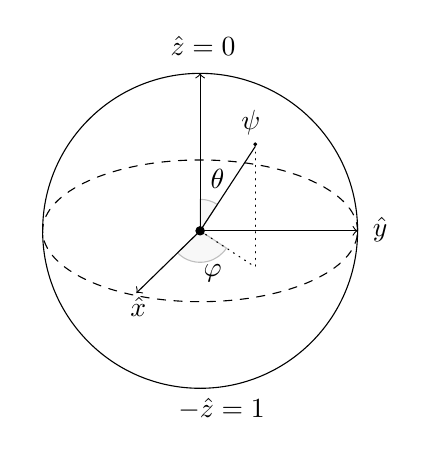
\begin{tikzpicture}[line cap=round, line join=round]
    \clip(-2.19,-2.49) rectangle (2.66,2.58);
    \draw [shift={(0,0)}, lightgray, fill, fill opacity=0.1] (0,0) -- (56.7:0.4) arc (56.7:90.:0.4) -- cycle;
    \draw [shift={(0,0)}, lightgray, fill, fill opacity=0.1] (0,0) -- (-135.7:0.4) arc (-135.7:-33.2:0.4) -- cycle;
    \draw(0,0) circle (2cm);
    \draw [rotate around={0.:(0.,0.)},dash pattern=on 3pt off 3pt] (0,0) ellipse (2cm and 0.9cm);
    \draw (0,0)-- (0.70,1.07);
    \draw [->] (0,0) -- (0,2);
    \draw [->] (0,0) -- (-0.81,-0.79);
    \draw [->] (0,0) -- (2,0);
    \draw [dotted] (0.7,1)-- (0.7,-0.46);
    \draw [dotted] (0,0)-- (0.7,-0.46);
    \draw (-0.08, -0.3)  node[anchor=north west] {$\varphi$};
    \draw (0.01,  0.9)   node[anchor=north west] {$\theta$};
    \draw (-1.01, -0.72) node[anchor=north west] {$\hat{x}$};
    \draw (2.07,  0.3)   node[anchor=north west] {$\hat{y}$};
    \draw (-0.5,  2.6)   node[anchor=north west] {$\hat{z}=\ket{0}$};
    \draw (-0.4,  -2)    node[anchor=north west] {$-\hat{z}=\ket{1}$};
    \draw (0.4,   1.65)  node[anchor=north west] {$\ket{\psi}$};
    \scriptsize
    \draw [fill] (0,0) circle (1.5pt);
    \draw [fill] (0.7,1.1) circle (0.5pt);
\end{tikzpicture}

    }{%
        Picture of a Bloch sphere.
        A generic state of a qubit can be written as
        $\ket{\psi} = \cos \frac{\theta}{2} \ket{0} + e^{i \varphi} \sin \frac{\theta}{2} \ket{1}$, so it is fully described by a two angles $\theta$ and $\phi$.
        For this reason, the Hilbert space of a qubit can be visualized as a two-dimensional sphere.%
    }
\end{figure}


The logical operators, or \emph{gates}, of classical computation are single-bit or double-bit functions that have only a single-bit output.
This makes classical computation \emph{non-reversible}\footnote{%
    There exist models of classical computation that are reversible, see \cite{fredkin1982logic}, which will not be discussed here and are not very common in every-day applications.
    In \cite{fredkin1982logic} a universal \emph{three-bits} gate is introduced that allows for reversible computation.%
}.
The idea behind quantum computing is to use the time-evolution of an ad-hoc quantum machine for performing computation.
Time-evolution is a \emph{unitary} process, which means that is reversible.
Hence, the non-reversible model of classical computation is not suited for quantum computing.
There is no one-to-one correspondence between the operations on a classical machine and those on a quantum machine.
Logical operations on a quantum computer, also called \emph{quantum gates}, have to implemented through \emph{unitary operators} that act on the quantum register.
A succession of logical operator, therefore, is equivalent to the product of these unitary operators.
This makes the whole computation a unitary process, hence reversible.

It is known, in classical computing, that only a minimal set of logical gates are actually needed in order to perform any computation.
For example, with a \texttt{NOT} gate and a \texttt{AND} gate is possible to implement every other possible logical function (actually only the \texttt{NAND} gate is necessary).
A similar result is true also for quantum computing \cite{barenco1995gates}.
One only needs a minimal set of quantum gates in order to implement any unitary operators with arbitrary precision.
Similar to the classical case, for quantum computing we only need single-qubit and two-qubits gates.
The two-qubits gates have an important role, because they allow to introduce \emph{entanglement}, which is the secret ingredient that makes quantum computing distinct from classical computing.
This minimal set usually entails a set of single-qubit and one two-qubits entangling gate (like the \texttt{CNOT} gate).
In Fig.~\ref{fig:quantum_gates} some example of quantum gates are shown, while in Fig.~\ref{fig:quantum_fourier} an example of a quantum circuit can be found.

\begin{figure}[t]
    \SideFigure[label=fig:quantum_gates, desc={Example of quantum gates}]{
        \begin{tikzpicture}[
    scale=0.5,
    gate/.style = {draw=black, fill=white, thick, minimum size=0.6cm, inner sep=0pt, font=\footnotesize}
    ]
    \draw (0, 0) -- ++(3, 0) node [right=5pt] {$\frac{1}{\sqrt{2}} \begin{pmatrix} 1 & 1 \\ 1 & -1 \end{pmatrix} $};
    \node[gate] at (1.5, 0) {$H$};

    \draw (0, -3) -- ++(3, 0) node [right=5pt] {$ \begin{pmatrix} 1 & 0 \\ 0 & e^{i 2 \pi / 2^k} \end{pmatrix}$};
    \node[gate] at (1.5, -3) {$R_k$};


    \draw (0, -6) -- ++(3, 0);
    \draw (0, -7.5) -- ++(3, 0);
    \draw[cline] (1.5, -6) -- ++(0, -1.5) node {$\bigoplus$};
    \node[control] at (1.5, -6) {};
    \node[right=5pt] at (3, -6.75) {$\begin{pmatrix}
                1 & 0 & 0 & 0 \\
                0 & 1 & 0 & 0 \\
                0 & 0 & 0 & 1 \\
                0 & 0 & 1 & 0
        \end{pmatrix}$};
\end{tikzpicture}


    }{
        Examples of quantum gates.
        From top to bottom:
        \emph{(i)} Hadamard gate $H$;
        \emph{(ii)} Phase gate $R_k$;
        \emph{(iii)} \texttt{CNOT} (controlled \texttt{NOT}) gate.
    }
\end{figure}

\medskip

Even though it has been proven that ``anything'' can be simulated on a quantum computer \cite{lloyd1996simulator}, not all unitary operations can be simulated \emph{efficiently}.
The time-evolution of the target quantum system requires \emph{digitalization}, which means that it has to be decomposed in smaller steps in order to be encodable as a sequence of quantum gates.
This is possible to an arbitrary precision thanks to the Trotter-Suzuki product formula for the exponentiation of complex matrices:
\begin{equation}
    e^{A + B}  = \lim_{n \to \infty} \qty( e^{A/n} e^{B/n} )^n.
\end{equation}
In most physically interesting case, the Hamiltonian is a sum of non-commuting terms:
\begin{equation*}
    H = \sum_{l} H_{l},
\end{equation*}
where $\comm{H_l}{H_{l^{\prime}}} \neq 0$ for $l \neq l^{\prime}$.
In the case of a time-independent Hamiltonian, the time-evolution operator is given by
\begin{equation}
    U(t) = e^{-i t \sum_{l} H_l }
    \quad \text{such that} \quad
    U(t) \ket{\psi(0)} = \ket{\psi(t)}.
    \label{eq:time_evolution_operator}
\end{equation}
In order to implement \eqref{eq:time_evolution_operator} on a quantum operator, the time-evolution has to be divided in $N$ steps of length $\Delta t$, such that $t = N \Delta t$ and $U(t) \simeq (U(\Delta t))^N$.
For each single time step we can apply the first-order Trotter-Suzuki formula \cite{nielsen2010quantum, somma2002simulating} for the time-evolution operator:
\begin{equation}
    U(\Delta t)
    = e^{- i \Delta t \sum_{l} H_l}
    = \prod_{l} e^{-i \Delta t H_l} + O(\Delta t^2).
    \label{eq:trotter_time_evolution}
\end{equation}

The drawback of Trotterization is that high accuracy comes at the cost of very small $\Delta t$ and therefore a very large number of quantum gates.
The scheme used in \eqref{eq:trotter_time_evolution} has some shortcomings, that can be improved with higher order decompositions that will necessarily introduce more complexities in the quantum circuit.
Moreover, some other types of methods have to be used in the case of time-dependent Hamiltonians \cite{wiebe2011simulation}.

\medskip

It should be stressed that we are still far from perfect digital quantum computation.
A typical quantum computer is affected by noise due to its interaction with the environment.
The effect of noise can corrupt the state of the quantum register, by flipping or dephasing the qubits for example.
Furthermore, interaction with an external environment will necessarily lead to \emph{decoherence} where all the ``quantumness'' of the system is lost \cite{zurek1991decoherence, schlosshauer2014decoherence, schlosshauer2019decoherence}.

It becomes clear that error correction is a necessity for \emph{fault-tolerant quantum computing} \cite{preskill1997faulttolerant, shor1996faulttolerant} but it can greatly increase the number of qubits needed for useful computations.
Indeed, it is said we are currently living in the \emph{noisy intermidiate-scale quantum} (NISQ) era of quantum computing \cite{preskill2018quantumcomputing}.
The term refers to moderately sized quantum computers (around 50--100 qubits) whose gates are still affected by noise but are not large enough to fully implement error correction.

\medskip

The typical setup for a digital simulation consists of three steps:
\begin{description}[font=\normalfont\itshape, labelsep=1.1em]
    \item[Initial-state preparation.] The quantum register is prepared in the initial state $\ket{\psi(0)}$.
        This step can be difficult by itself, and it is not always guaranteed that an efficient algorithm may exist.

    \item[Unitary evolution.] The circuit has to reproduce or simulate the action of a unitary operator $U$.
        This unitary operator is usually the time-evolution operator of the target system, which has to be decomposed in a sequence of smaller operation through trotterization, as explained before.

    \item[Final measurement.] After obtaining the wanted state $\ket{\psi(t)} = U \ket{\psi(0)}$, a \emph{measurement} is needed in order to extract relevant physical information.
        Instead of capturing the whole wave function $\ket{\psi(t)}$, with, for example, quantum tomography, one may proceed with the direct estimation of certain physical quantities, such as correlation functions or spectra of operators.
\end{description}


\begin{figure}[t]
    \centering
    \scalebox{0.75}{\begin{tikzpicture}[
    scale=0.5,
    font=\scriptsize,
    % gate/.style = {rounded corners=2pt, fill=white}
    ]
    \foreach \n/\y in {0/0, 1/1.5, 2/4, 3/5.5} {
        \node (q\n) at (0, -\y) {};
        \node (q\n end) at (25, -\y) {};
        % \path (q\n) edge (q\n end);
    }
    \node[left] at (q0) {$\ket{j_1}$};
    \node[left] at (q1) {$\ket{j_2}$};
    \node[left] at (q2) {$\ket{j_{n-1}}$};
    \node[left] at (q3) {$\ket{j_{n}}$};

    \node[right] at (q0end) {$\ket{0} + e^{i 2 \pi 0.j_1 \dots j_n} \ket{1}$};
    \node[right] at (q1end) {$\ket{0} + e^{i 2 \pi 0.j_2 \dots j_n} \ket{1}$};
    \node[right] at (q2end) {$\ket{0} + e^{i 2 \pi 0.j_{n-1} j_n} \ket{1}$};
    \node[right] at (q3end) {$\ket{0} + e^{i 2 \pi 0.j_n} \ket{1}$};

    \node[gate] at (1, 0) {$H$};
    \node[gate] at (3, 0) {$R_2$};
    \node[gate] at (6, 0) {$R_{n-1}$};
    \node[gate] at (8, 0) {$R_{n}$};

    \node[gate] at (10, -1.5) {$H$};
    \node[gate] at (13, -1.5) {$R_{n-2}$};
    \node[gate] at (15.5, -1.5) {$R_{n-1}$};

    \node[gate] at (19, -4) {$H$};
    \node[gate] at (21, -4) {$R_{2}$};

    \node[gate] at (23.5, -5.5) {$H$};

    \begin{scope}[on background layer]

        % circuit lines

        \draw (q0) -- (3.9, 0) coordinate (x);
        \draw[dotted] (x) -- (4.7, 0) coordinate (x);
        \draw (x) -- (q0end);

        \draw (q1) -- (3.9, -1.5) coordinate (x);
        \draw[dotted] (x) -- (4.7, -1.5) coordinate (x);
        \draw (x) -- (11, -1.5) coordinate (x);
        \draw[dotted] (x) -- (11.8, -1.5) coordinate (x);
        \draw (x) -- (17, -1.5) coordinate (x);
        \draw[dotted] (x) -- (17.8, -1.5) coordinate (x);
        \draw (x) -- (q1end);

        \draw (q2) -- (17, -4) coordinate (x);
        \draw[dotted] (x) -- (17.8, -4) coordinate (x);
        \draw (x) -- (q2end);

        \draw (q3) -- (17, -5.5) coordinate (x);
        \draw[dotted] (x) -- (17.8, -5.5) coordinate (x);
        \draw (x) -- (q3end);


        % control nodes and lines

        \node[control] at (3, -1.5) {};
        \draw[cline] (3, -1.5) -- (3, 0);
        \node[control] at (6, -4) {};
        \draw[cline] (6, -4) -- (6, 0);
        \node[control] at (8, -5.5) {};
        \draw[cline] (8, -5.5) -- (8, 0);

        \node[control] at (13, -4) {};
        \draw[cline] (13, -4) -- (13, -1.5);
        \node[control] at (15.5, -5.5) {};
        \draw[cline] (15.5, -5.5) -- (15.5, -1.5);

        \node[control] at (21, -5.5) {};
        \draw[cline] (21, -5.5) -- (21, -4);

    \end{scope}

\end{tikzpicture}
}
    \caption[Example of a quantum circuit]{
        Example of a quantum circuit.
        In particular this circuit executes the quantum Fourier transform \cite{nielsen2010quantum}.
        It uses some of the gates showed in Fig.~\ref{fig:quantum_gates}.
    }
    \label{fig:quantum_fourier}
\end{figure}


%
% SUBSECTION: Analog quantum simulations
%
\subsection{Analog quantum simulations}
\label{sub:analog_quantum_simulations}

Analog \ac{qs} is another type of approach to \ac{qs}, where one quantum system (the simulator) mimics or emulate another (the target) \cite{buluta2009simulators, wei1997simulation, arguello2019simulation, aspuruguzik2012photonic, blatt2012trappedions, bloch2012ultracold, houck2012superconducting, lewenstein2012ultracold}.
This approach is not based on building a universal machine, like a quantum computer, that can emulate any other system.
Instead, it focuses on recreating the features, or a subset of relevant features, of a chosen class of models in order to compute some physically relevant quantities.

Analog \ac{qs} follows the idea of \emph{analog computation}, where an experimental device is conceived for executing a specific algorithm, meaning that it is a specialized machine with some degree of controllability.
Analog computation is not a new idea, rather it is the oldest type of computing devised by mankind, and analog machines are the earliest types of computers to ever be used \cite{kendon2010quantum}.
Some historical examples can be the astrolabe for plotting the heavens (around 200 BC), the Antikythera mechanism for predicting astronomical routes (around 150 BC), or the mechanical differential analyser for integrating differential equations (around 1876) \cite{thomson1876integration}.

In an analog simulation, the Hamiltonian of the target $H^{\text{targ}}$, is directly mapped onto the Hamiltonian of the simulator, $H^{\text{sim}}$:
\begin{equation*}
    H^{\text{targ}} \longleftrightarrow H^{\text{sim}}.
\end{equation*}
Obviously, this is possible only if there is a mapping between the system and the simulator.
If $\ket{\phi(0)}$ is the initial state of the target, then it can be mapped to the initial state $\ket{\psi(0)}$ of the simulator, via an operator $\mathcal{O}$, i.e.~$\ket{\psi(0)} = \mathcal{O} \ket{\phi(0)}$.
Next, the simulator would perform the desired time evolution $U(t) \ket{\psi(0)} = \ket{\psi(t)}$.
The result then can be mapped back to a state of the target system via $\mathcal{O}^{-1}$, i.e.~$\mathcal{O}^{-1}\ket{\psi(t)} = \ket{\phi(t)}$.
In this case the Hamiltonians would be related by the mapping $\mathcal{O}$, $H^{\text{sim}} = \mathcal{O} H^{\text{targ}} \mathcal{O}^{-1}$.
Note that the simulator may only partly reproduce the dynamics of the target, or simulate some effective description of the system.
The choice of the mapping depends on what needs to be simulated and on the capabilities of the simulator \cite{georgescu2014simulation}.
Finding the mapping in an analog \ac{qs} might look, at first, simpler than finding the most efficient gate decomposition of a Hamiltonian, but it is not always true and there are no recipes ready for constructing these mappings in a general case.
% The obvious drawback of AQS is that the quantum simulators are problem specific, but on the other hand, given that they do not require a full quantum computer, they are more feasible in the near-term.

Initial state preparation is not such a topic in analog \ac{qs}, as it is in digital \ac{qs}.
This is based on the assumption that the target system and the simulator are presumed to be very similar.
It is expected that the preparation of the initial state can occur naturally in processes mimicking the natural relaxation of the simulated system to an equilibrium state.
Moreover, analog \ac{qs} has the natural advantage that physical quantities can be measured directly, without the need of special schemes like in digital \ac{qs}, which can yield direct information about the target system \cite{hauke2012simulators}.

One important advantage of analog \ac{qs} is that fact that it does not require a fully fledged quantum computer.
In fact, the simulator does not even need to be a quantum computer at all.
This possibly makes analog \ac{qs} much more achievable from the experimental point of view.
Many different platforms are already available (see also Fig.~\ref{fig:analog_simulators}):
\begin{itemize}
    \item ultracold atoms and molecules \cite{lewenstein2012ultracold, bloch2012ultracold, bloch2008ultracold, lin2009ultracold, muller2012ions, aidelsburger2011ultracold};
    \item trapped ions \cite{blatt2012trappedions, muller2012ions, johanning2009ions, schneider2012ions};
    \item photons \cite{aspuruguzik2012photonic, angelakis2017quantum};
    \item polaritons \cite{angelakis2017quantum, hartmann2006polaritons};
    \item nuclear magnetic resonance (NMR) systems \cite{somaroo1999simulation, tseng1999nmr};
    \item artificial lattices \cite{singha2011lattice};
    \item superconducting qubits \cite{houck2012superconducting, makhlin2001superconducting, devoret2004superconducting, you2005superconducting, pritchett2010superconducting}.
\end{itemize}

Analog \ac{qs} can be useful even in the presence of errors, up to a certain tolerance level, because it would still be able to give qualitative answers.
Suppose one is interested in knowing if whether a certain set of physical conditions leads to a given quantum phase transition.
Even without the full quantitative description or the perfect tuning of the control parameters, an analog simulator would, potentially, still be able to show the presence or not of a phase transition.
Furthermore, due to the analog nature of these simulators, standard error correction and fault tolerance are not allowed \cite{hauke2012simulators}, while the level of controllability depends on the type of platform used.
For example, in the case of ultracold atoms in optical lattices the typical control parameters involve lattice parameters (laser wavelength, geometry, dimensionality, etc\dots), temperature and other thermodynamical control parameters, as well as atomic interaction strength \cite{lewenstein2012ultracold}.


\begin{figure}[t]
    \centering
    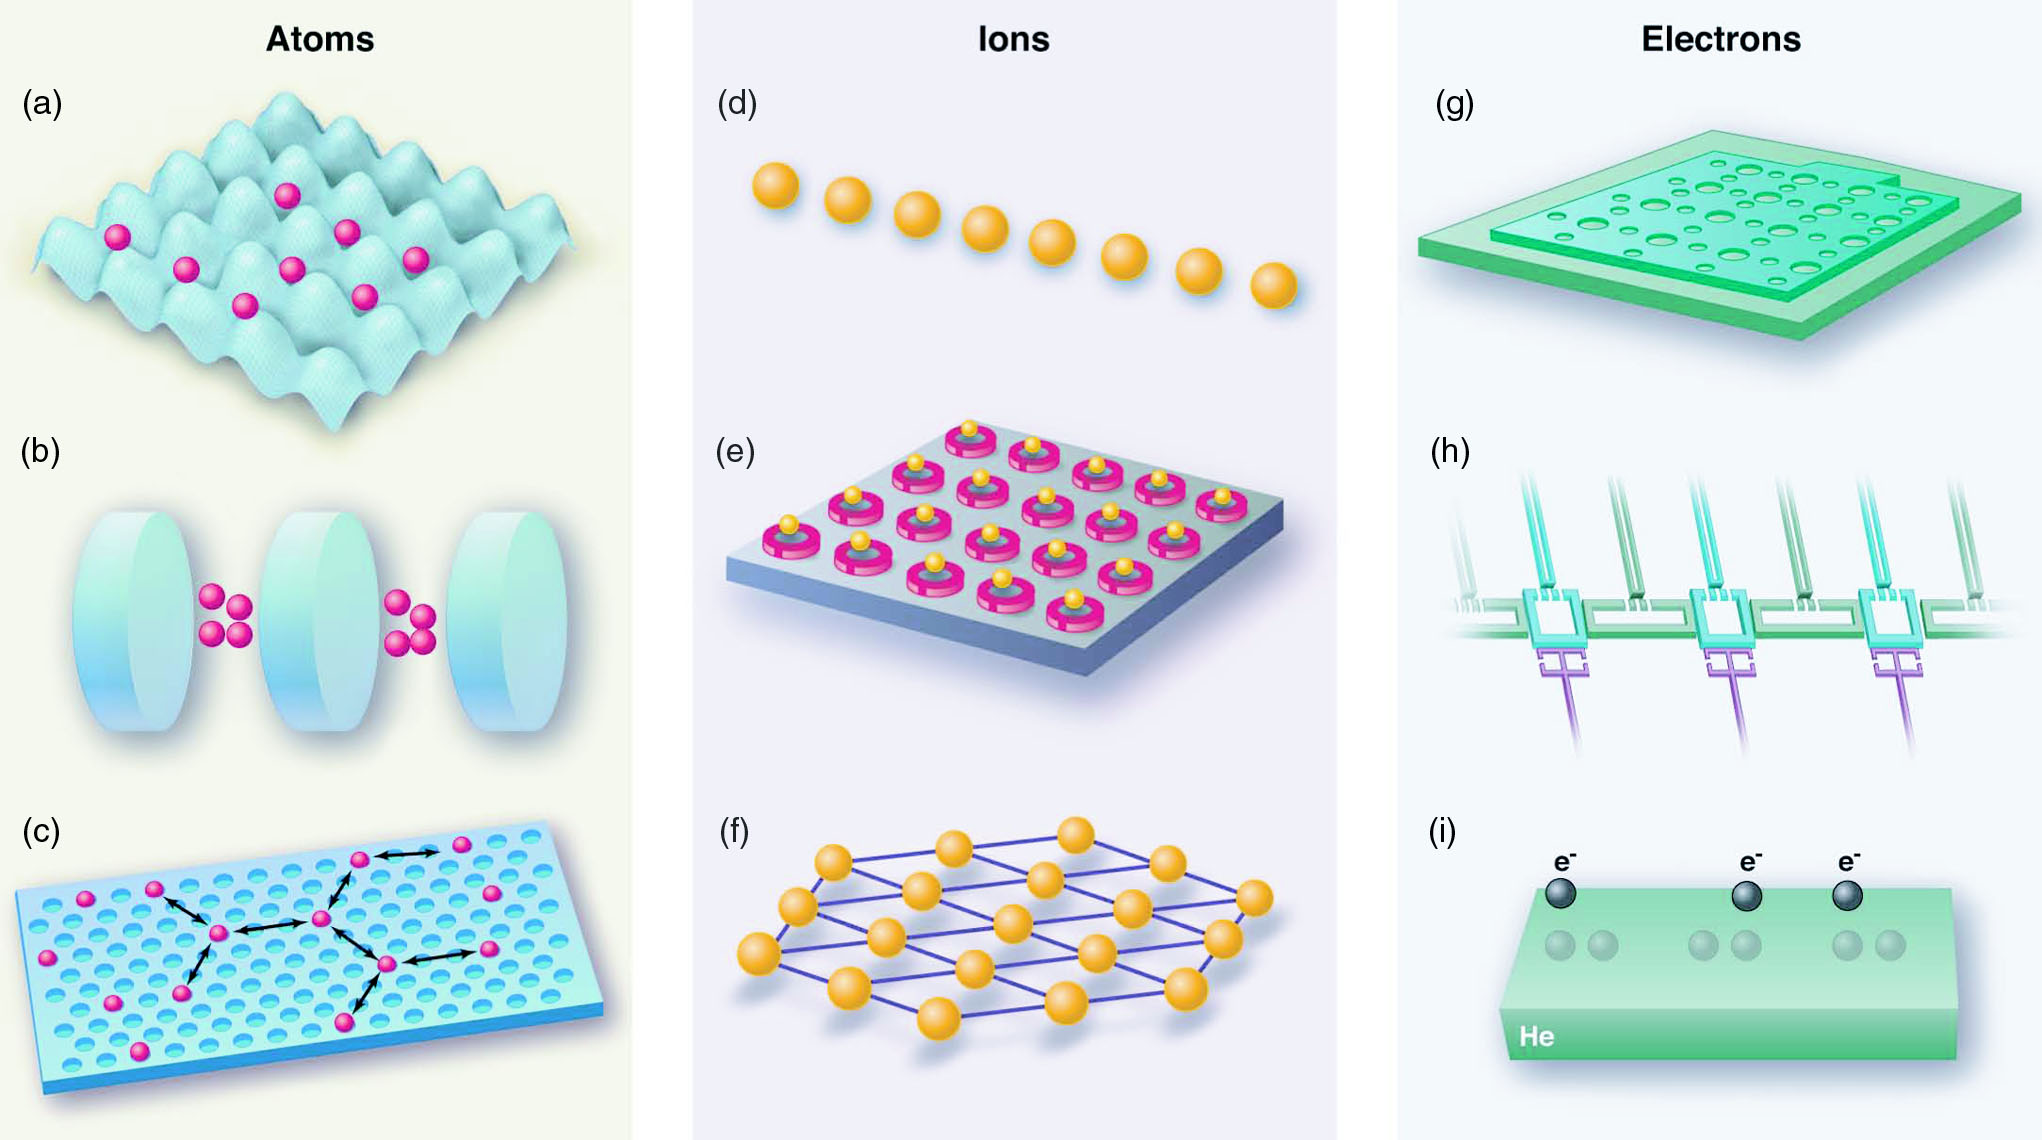
\includegraphics[width=\textwidth]{assets/figures/quantum_simulators.png}
    \caption[Examples of analog quantum simulators]{
        Picture from \cite{buluta2009simulators}.
        Examples of analog quantum simulators:
        \emph{(a)} atoms in optical lattices,
        \emph{(b)} one-dimensional or
        \emph{(c)} two-dimensional arrays of cavities;
        \emph{(d)} ions in linear chains,
        \emph{(e)} two-dimensional arrays of planar traps, or
        \emph{(f)} two-dimensional Coulomb crystal;
        \emph{(g)} electrons in quantum dot arrays created by a mesh gate,
        \emph{(h)} in arrays of superconducting circuits, or
        \emph{(i)} trapped on the surface of liquid helium.
        For more details see \cite{buluta2009simulators, georgescu2014simulation}.
    }
    \label{fig:analog_simulators}
\end{figure}


%
% SUBSECTION: Quantum-inspired algorithms
%
\subsection{Quantum-inspired algorithms}
\label{sub:quantum_inspired_algorithms}

Classical simulations of quantum systems are usually done using one of the following methods \cite{hauke2012simulators}:
\begin{itemize}[itemsep=0pt]
    \item Quantum \ac{mc}.
    \item Systematic perturbation theory.
    \item \Ac{ed}.
    \item \Ac{dmrg}.
\end{itemize}
Each of these methods has its problems.
Quantum \ac{mc} methods can work with large systems but fails for fermionic systems due to the sign problem \cite{sandvik2010computational, troyer2010computational}.
Perturbation theory is applicable only when there is a small coupling constant, so it fails for strongly interacting systems.
\Ac{ed} works only for rather small systems \cite{sandvik2010computational, troyer2010computational}.
\Ac{dmrg} is a variation methods that has been proven to work also for strongly interacting systems \cite{schollwock2011dmrg, mcculloch2007dmrg, dechiara2008dmrg}.
It has been proven to be of great success for one-dimensional systems, while for two-dimensional models it can be quite limited \cite{stoudenmire2012dmrg}.

Thanks to the development of quantum information, new \emph{classical algorithms} have been invented for the simulation of many-body systems that much more exploit the quantum nature of these systems.
One of the most groundbreaking example of quantum-inspired algorithms is the use of \emph{\ac{tn} states} \cite{orus2014tensor, verstraete2004algo, verstraete2008tensor, verstraete2004dmrg, vidal2008simulation, cirac2009tensor}.
\Acp{tn} make it possible to ``compress'' the information about a many-body wave function by expressing it as a \emph{contraction} of a network of tensors (as suggested by the name).

In details, to each physical site we associate a tensor with a number of indices (or legs).
One of these indices is called the \emph{physical index} of the tensors, which runs over the basis of the local Hilbert space.
The other indices are \emph{auxiliary indices}, their dimension is governed by a parameter $\chi$ called the \emph{bond dimension} and are ``connected'' to other sites.
Roughly speaking, these auxiliary indices encodes the entanglement information between the connected sites.

To make it more clear, consider a one-dimensional open chain (with $L$ sites), where each site has a $d$-dimensional local Hilbert space with basis $\{\ket{i}, i = 1,\dots,d\}$.
A general global state $\ket{\Psi}$ of the whole chain can be written as
\begin{equation}
    \ket{\Psi} = \sum_{i_1, \dots, i_L} C_{i_1, \dots, i_L} \ket{i_1 \cdots i_L}.
\end{equation}
It is easy to see that the whole state is encoded in the $L$-th order tensor $C_{i_1, \dots, i_L}$ and the indices $i_n$ are called physical indices.
Notice that $C_{i_1, \dots, i_L}$ has $d^L$ entries.
Through \emph{\ac{svd}} it is possible to factorize the tensor $C_{i_1, \dots, i_L}$ into $L$ tensors $A^{i_n}$, one for each site \cite{schollwock2011dmrg}:
\begin{equation}
    C_{i_1, \dots, i_L}
    = \sum_{\alpha_1, \dots, \alpha_{L-1}}
    A^{i_1}_{\alpha_1}
    A^{i_2}_{\alpha_1, \alpha_2}
    \cdots
    A^{i_{L-1}}_{\alpha_{L-2}, \alpha_{L-1}}
    A^{i_L}_{\alpha_{L-1}}.
    \label{eq:mps_decomposition}
\end{equation}
The indices $\alpha_n$ are called auxiliary indices.

The order of $\alpha_n$ depends on the number of Schmidt eigenvalues of the bipartition that separates the first $n$ sites from the rest.
In other words, it depends on the entanglement entropy between the first $n$ sites of the chain and the rest.
Not all the Schmidt eigenvalues are of the same importance, therefore each tensor $A^{i_n}$ can be optimized by discarding the Schmidt eigenvalues under a certain threshold.
In this way we compress the wave-function, by preserving the information that best represent the entanglement in the state.
The order of the indices $\alpha_n$ is called the \emph{bond-dimension}, often denoted $\chi$, and it is this parameter that fine tunes the amount of entanglement.
Notice that with $\chi$ fixed, the right hand side of \eqref{eq:mps_decomposition} has only around $L d \chi^2$ entries, which scales better that $d^L$.
If the system has a finite amount of entanglement, then there is an optimal value for the bond dimension $\chi$.
This would mean that we do not really need all the $d^L$ entries of $C$, but the $L d \chi^2$ entries of \eqref{eq:mps_decomposition} are sufficient to faithfully represent $\ket{\Psi}$.

For a large class of physically relevant models, the ground state is gapped and has, in a certain sense, a finite amount of entanglement, which can be explained by the finite correlation length.
This fact is expressed by the so-called \emph{area law}, where the entanglement between two partitions of the system grows with size of the boundary, the area between the two partitions, and not with the size of the partition itself \cite{vidal2003arealaw, calabrese2004qft, calabrese2009cft, srednicki1993area, plenio2005area}.
The main advantage of \ac{tn} methods is their ability to capture this area law, which lead to an efficient computation of the ground states of these models.

\Acp{tn} were first inspired by the ground state of the AKLT model \cite{affleck1987aklt}, and from there different types \acp{tn} were developed.
The paradigmatic example of \acp{tn} are the \emph{\acp{mps}} in one-dimension \cite{vidal2008simulation, schollwock2011dmrg}, and the \emph{\acp{peps}} in two dimensions \cite{verstraete2004algo, jordan2008ipeps}.
Some other variants of \acp{tn} exists, like \emph{Tree \acp{tn}} \cite{tagliacozzo2009tree, fannes1992trees} or \emph{\ac{mera}} \cite{evenbly2013mera, vidal2007entanglement, evenbly2009entanglement}.

\begin{figure}[t]
    \centering
    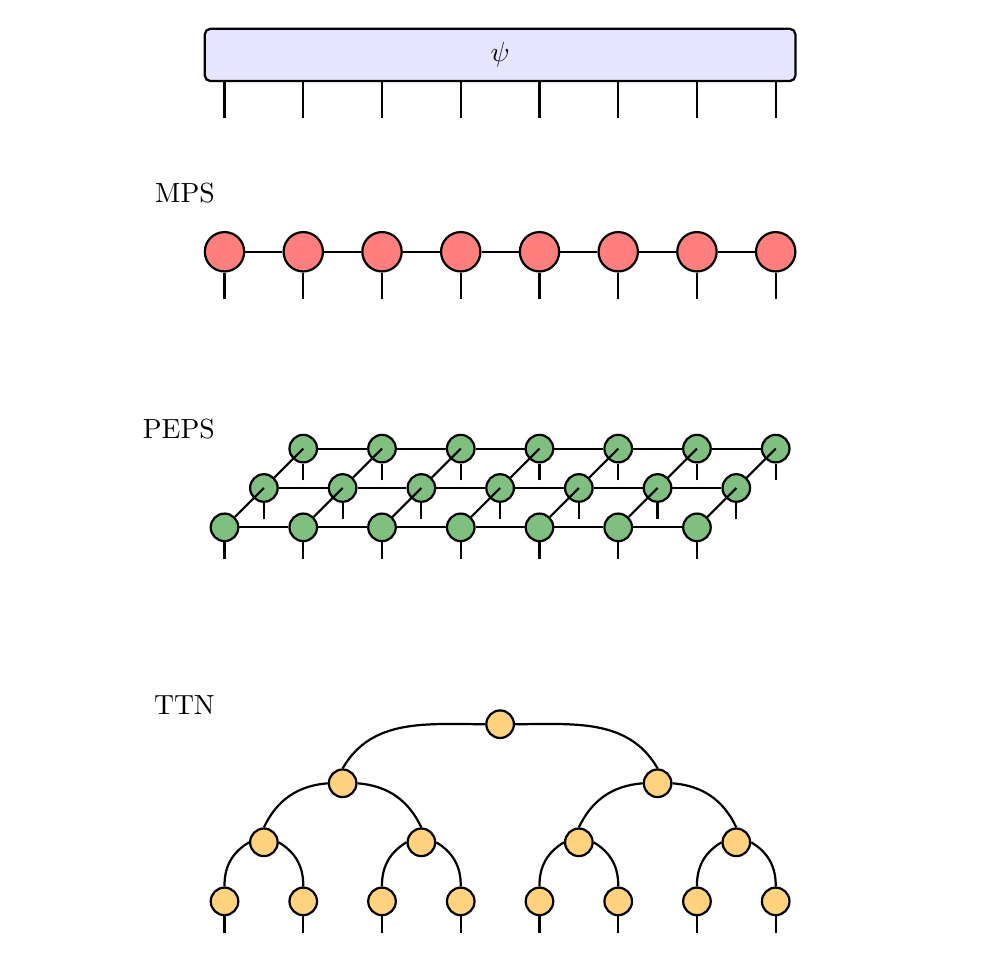
\begin{tikzpicture}[
    index/.style = {thick},
    mps tensor/.style = {circle, draw, thick, fill=Red, fill opacity=0.5, minimum size=0.5cm, inner sep=0pt},
    peps tensor/.style = {circle, draw, thick, fill=Green, fill opacity=0.5, minimum size=0.35cm, inner sep=0pt},
    ttn tensor/.style = {circle, draw, thick, fill=Orange, fill opacity=0.5, minimum size=0.35cm, inner sep=0pt}
    ]
    % Generic quantum state
    \node[
    rectangle,
    minimum width=7.5cm,
    draw,
    thick,
    inner sep=5pt,
    rounded corners=2pt,
    fill=Blue,
    fill opacity=0.1,
    font=\normalsize,
    text=black,
    text opacity=1
    ] (psi) at (0, 0) {$\ket{\psi}$};
    \foreach \n in {-3.5, -2.5, ..., 3.5} {
        \draw[index] (\n, -0.8) -- (\n, -0.8 |- psi.south);
    }

    % MPS
    \begin{scope}[yshift=-2.5cm, xshift=-3.5cm]
        \foreach \n in {0, ..., 7} {
            \node[mps tensor] (mps \n) at (\n, 0) {};
            \draw[index] (\n, -0.6) -- (\n, -0.6 |- mps \n.south);
        }
        \foreach \n in {0, ..., 6} {
            \pgfmathtruncatemacro{\m}{\n + 1}
            \draw[index] (mps \n.east) -- (mps \m.west);
        }
    \end{scope}

    % PEPS
    \begin{scope}[yshift=-6cm, xshift=-3.5cm]
        \foreach \y/\n in {0/0, 0.5/1, 1/2} {
            \foreach \x in {0, ..., 6} {
                \node[peps tensor] (peps \x \n) at (\x + \y, \y) {};
                \draw[index] (\x + \y, \y-0.4) -- (\x + \y, \y-0.4 |- peps \x \n.south);
            }
            \foreach \x in {0, ..., 5} {
                \pgfmathtruncatemacro{\w}{\x + 1}
                \draw[index] (peps \x \n.east) -- (peps \w \n.west);
            }
        }
        \foreach \n in {1, 2} {
            \pgfmathtruncatemacro{\m}{\n-1}
            \foreach \x in {0, ..., 6} {
                \draw[index] (peps \x \n.center) -- (peps \x \m.north east);
            }
        }
    \end{scope}

    % TTN
    \begin{scope}[yshift=-10.75cm, xshift=-3.5cm]
        % level 0
        \foreach \n in {0, ..., 7} {
            \node[ttn tensor] (ttn 0 \n) at (\n, 0) {};
            \draw[index] (\n, -0.4) -- (\n, -0.4 |- ttn 0 \n.south);
        }

        % level 1
        \foreach \n in {0, ..., 3} {
            \pgfmathsetmacro{\x}{2 * \n + 0.5}
            \node[ttn tensor] (ttn 1 \n) at (\x, 0.75) {};
        }

        % level 2
        \foreach \n in {0, 1} {
            \pgfmathsetmacro{\x}{4 * \n + 1.5}
            \node[ttn tensor] (ttn 2 \n) at (\x, 1.5) {};
        }

        % level 3
        \node[ttn tensor] (ttn 3) at (3.5, 2.25) {};

        % indices
        \foreach \n in {0, ..., 3} {
            \pgfmathtruncatemacro{\a}{2 * \n}
            \pgfmathtruncatemacro{\b}{2 * \n + 1}
            \draw[index] (ttn 0 \a.north) edge[bend left ] (ttn 1 \n.west);
            \draw[index] (ttn 0 \b.north) edge[bend right] (ttn 1 \n.east);
        }
        \foreach \n in {0, 1} {
            \pgfmathtruncatemacro{\a}{2 * \n}
            \pgfmathtruncatemacro{\b}{2 * \n + 1}
            \draw[index] (ttn 1 \a.north) edge[bend left ] (ttn 2 \n.west);
            \draw[index] (ttn 1 \b.north) edge[bend right] (ttn 2 \n.east);
        }
        \draw[index] (ttn 2 0.north) edge[out=60, in=180] (ttn 3.west);
        \draw[index] (ttn 2 1.north) edge[out=120, in=0] (ttn 3.east);
    \end{scope}

    % Labels
    \node[anchor=south east] at (-3.5, -2) {MPS};
    \node[anchor=south east] at (-3.5, -5) {PEPS};
    \node[anchor=south east] at (-3.5, -8.5) {TTN};

    % for centering
    \path (-6, 0) -- (6, 0);
\end{tikzpicture}


    \caption{Examples of \acp{tn}}
\end{figure}

\Ac{tn} methods can still have some shortcomings.
They work especially well for one-dimension gapped systems, but then can become challenging to make them work efficiently for gapless systems or higher dimensions.
When a system is in a gapless phase, the correlation length diverges, which leads to changes in the structure of entanglement.
This is best captured by the behaviour of entanglement entropy in massive or massless one-dimensional systems \cite{calabrese2004qft, calabrese2009cft}.
In a massive and gapped theory, the entanglement entropy is directly proportional to number of boundary points, irregardless of the subsystem size (as long as it is larger then the correlation length).
On the other hand, in a massless and critical phase the entanglement entropy has a direct dependence on the size of the subsystem.
Therefore, it is easy to see that in a critical phases the bond-dimension would, potentially, need to increase with the system size in order to effectively capture the ground-state wave-function.
Another shortcoming is the computational complexities of tensor contractions in dimensions higher than one.
This is because the order of each tensor increases with the dimensionality of the system, which lead to higher computational costs when performing calculations \cite{orus2014tensor}.
